\section{Results} \label{sec:Results}

% Methodology
In this section, we report experimental results of urban traffic-light control system based on MQTT protocol. We report the limitations of our solution. To test the efficiency of MQTT protocol, we made 2 scenarios, in the first scenario, the frequency  packets sending  is 1 packet per 10s, the second scenario, the frequency  packets sending  is 1 packet per 1s. The measured delays have been taken into account between the Middleware (Edge) to the Cloud platform (Ubidots) throughout the Internet. Note that we don't know the routes and the routers that our packets will go through. We measured the Round Trip Time (RRT) for the packets exchanged between the two sides. In each scenario, more than 100 values have been taken. Tests have been reproduced for two different hours and days.

%\Figure{!htb}{1}{cdf_distribution.pdf}{Normal,Gamma and Logistic distribution}
\begin{figure}[!htb]
\centering
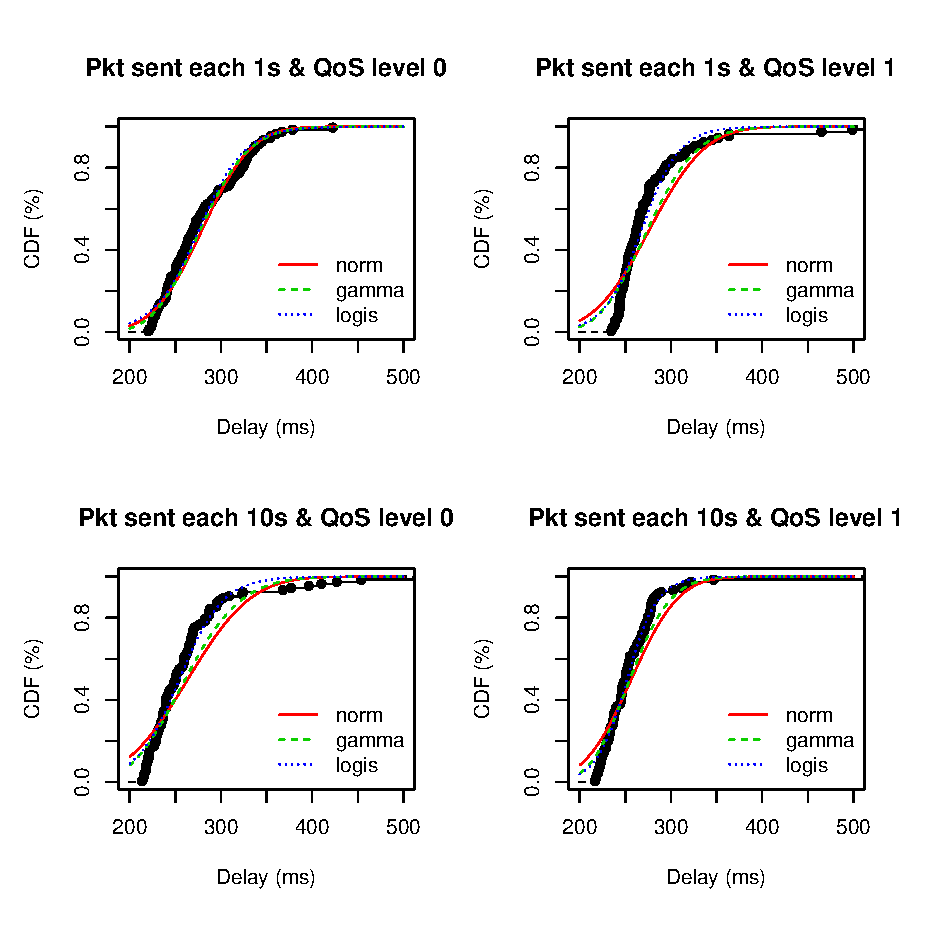
\includegraphics[width=\columnwidth]{Figures/distributions_v3.eps}
\caption{Normal, Gamma and Logistic distribution}
\label{fig:cdf_distribution.pdf}
\end{figure}

Fig. \ref{fig:cdf_distribution.pdf} shows the measured Cumulative Distribution Function (CDF) of RTT delays for the two levels of QoS, levels 1 and 2. We consider three probabilistic distribution functions (Normal, Gamma and Logistic) in the experimental results in order to characterize MQTT performance. The obtained correlation allows us to define a representative empirical model. Table \ref{table:correlation} details the results of a correlation matrix between distributions and experimental results. We can see that logistic distribution \cite{STEPHENS1979} fits better with our measured RTT values for the two scenarios. The standard logistic law is of parameters 0 and 1. Its distribution function of a random variable $x$ is the sigmoid following the expression:

\begin{equation}
F(x) = \frac{1}{1 + e^{-x}} \mbox{,where } x\in \left[ -\infty, +\infty\right]
\end{equation}
%\Equation{1}{F(x) = \frac{1}{1 + e^{-x}} \mbox{, where } x\in \left[ -\infty, %+\infty\right] } 

%Results show that packet delays in both scenarios with the level of QoS match better the logistic distribution than the tow other distributions.
%
%\blue{To study the behavior of packet delays in each scenario,
%	we select the best distribution that fit the round trip time (RTT) of packets,
%	we choose 3 common distributions normal,
%	gamma and logistic distribution shown in figure \ref{fig:cdf_distribution.pdf}.
%Table \ref{table:correlation} shows the correlation matrix between distributions and scenarios used in our study.
%Results show that packet delays in both scenarios with the level of QoS match better the logistic distribution than the tow other distributions.
%The standard logistic law is the logistic law of parameters 0 and 1, its distribution function is the sigmoid: 
%\Equation{1}{F(x) = \frac{1}{1 + e^{-x}}}
%}

\begin{table} [!htb]
\caption{Correlation between distributions and empirical results}
\centering
  \begin{tabular}{ | c | c | c | c | }
    \hline
	\                    & norm      & gamma    & logis         \\\hline 
	1s  with QoS level 1 & 172.12074 & 175.2950 & \bf{185.4433} \\\hline 
	1s  with QoS level 2 & 159.59630 & 172.8193 & \bf{189.7002} \\\hline 
	10s with QoS level 1 & 146.85668 & 161.2369 & \bf{175.3682} \\\hline 
	10s with QoS level 2 & 176.28502 & 192.6108 & \bf{204.3235} \\\hline
  \end{tabular}
\label{table:correlation}
\end{table}

%\Table{|c|c|c|c|}{correlation}{Matrix of correlation between distribution and empirical results }{
%	\                    & norm      & gamma    & logis         \\\hline 
%	1s  with QoS level 0 & 172.12074 & 175.2950 & \bf{185.4433} \\\hline 
%	1s  with QoS level 1 & 159.59630 & 172.8193 & \bf{189.7002} \\\hline 
%	10s with QoS level 0 & 146.85668 & 161.2369 & \bf{175.3682} \\\hline 
%	10s with QoS level 1 & 176.28502 & 192.6108 & \bf{204.3235} \\\hline
%}

\begin{figure}[!htb]
\centering
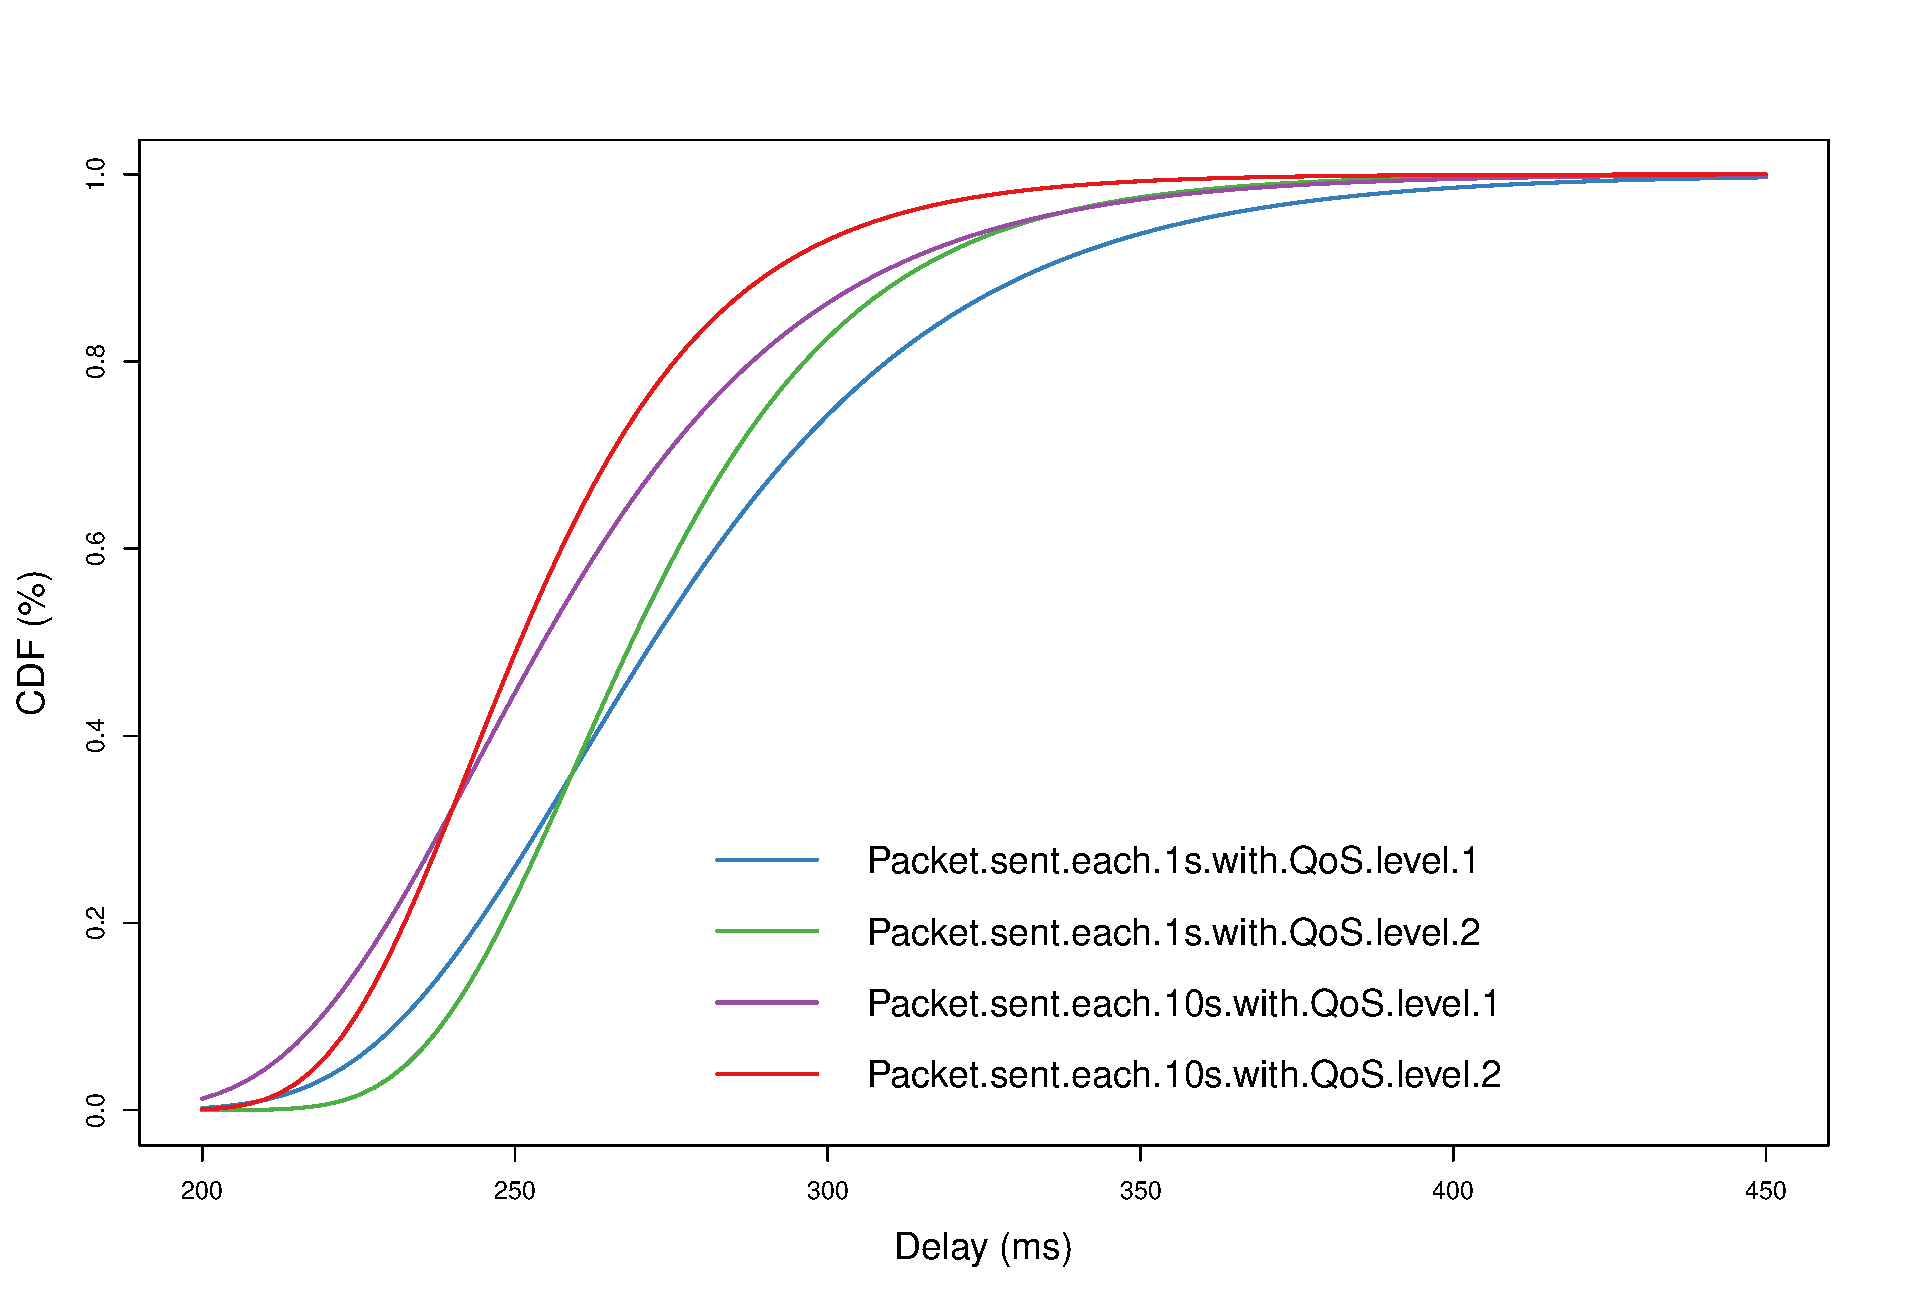
\includegraphics[width=3.5in]{Figures/cdf_v3.eps}
\caption{Cumulative distribution function of RTT delay for two QoS levels}
\label{fig:cdf.pdf}
\end{figure}

Fig.
\ref{fig:cdf.pdf} highlights the empirical model of CDF featuring the RTT of MQTT protocol.
As can be seen,
	RTT protocol is more efficient when the number of packets is greater than 35\% of the total number of packets sent.
This can be explained by the fact that priority queues are useful when queues of QoS are full.
In that case,
	the packets with a highest priority level will reach their destination with low latency.
Furthermore,
	when we increase the number of packets sent to Ubidots at one per second,
	the MQTT still offers the same efficiency with suitable delays.
The found latency of up to 400 ms would be problematic for real world safety applications which require at most 100 ms \cite{Chen2017}.
 
Although our Mockup is innovative by combining IEEE 802.15.4, 6LowPAN,
	MQTT protocol and Edge Computing,
	the performances of our solution depend on external parameters.
These parameters are related to Internet Service Provider and all packet's routes throughout Internet network from the Middleware to Ubidots.
Thus,
	real implementation of such a system should be done by introducing a private Cloud near data sources.


